\documentclass[12pt, a4paper, twoside, ngerman, openright, headsepline=true, footsepline=false]{scrbook}

% Präambel --> Nutzereingaben, Pakete und definierte Code-Darstellungen werden geladen.
% =======================================================================================
% Bitte die Angaben in den hintersten Klammern eintragen!
% Beispiel: \newcommand{\art}{Bachelorarbeit}

% Angaben für das Deckblatt
% ======================================================================================================
\newcommand{\art}{Bachelor-Teamprojekt}
\newcommand{\thema}{Analyse, Design und Implementierung von unterschiedlichen Generative Adversarial Network Architekturen im Bereich der Bildverarbeitung}
\newcommand{\themaEnglisch}{Analysis, design and implementation of different Generative Adversarial Network architectures in the field of image processing} % Titel auf englisch
\newcommand{\autor}{Elisa Du, Marcel Hoffmann}
\newcommand{\matrikel}{976090, 973043}
\newcommand{\prof}{Prof. Dr. rer. nat. E.-G. Haffner}
\newcommand{\betreuer}{Paul Fuhrmann} %bei Arbeit an der Hochschule weglassen
\newcommand{\abgabedatum}{01. Dezember 2023}


% Layout-Einstellungen
% ======================================================================================================
% Hier kann über die Angabe eines Zahlenwertes festgelegt werden, ob die Kapitel einen schwarzen Balken mit weißer Kapitelnummerierung am rechten Rand der rechten Seiten haben sollen oder nicht.
% Damit die Kapitelbalken angezeigt werden muss dem Zähler "kb" die Zahl 1 zugewiesen werden (\setcounter{kb}{1}). Damit die Kapitelbalken nicht erscheinen muss dem Zähler "kb" die Zahl 0 zugewiesen werden (\setcounter{kapitelbalken}{0}).
\newcounter{kb}
\setcounter{kb}{1}

% Hier kann eingestellt werden, ob der Anhang Kapitelbalken haben soll. 
\newcounter{akb}
\setcounter{akb}{1}
% Diese Datei "b_packages.tex" ist dafür gedacht alle Packages einzubinden, die benötigt werden. Außerdem werden einige Einstellungen vorgenommen.

%=== Einstellungen ==============================================
% Erstzeileneinzug ausschalten
\setlength{\parindent}{0cm}

%=== Text- und Sprachpackages ===================================
% Setzt die Inputcodierung zu utf8
\usepackage[utf8]{inputenc}
% korrekte Silbentrennung für Westeuropäische Sprachen
\usepackage[T1]{fontenc}

% neue deutsche Rechtschreibung, Anführungszeichen; als zweite Sprache wird Englisch verwendet
\usepackage[main=ngerman, english]{babel}

%=== Packages zum Layout des Dokuments =========================
% Stellt die Ränder der Seiten ein
\usepackage[top=4cm, bottom=3cm]{geometry}

% Stellt die Möglichkeit zum Spezifizieren und Definieren von Farben zur Verfügung.
\usepackage{xcolor}
\definecolor{HSTmint}{HTML}{8FD6BD}     % Mint-Farbton der Hochschule-Trier
\definecolor{HSTorange}{HTML}{BE531C}   % Orange-Farbton der Hochschule-Trier
\definecolor{HSTgelb}{HTML}{D9C756}     % Senfgelb-Farbton der Hochschule-Trier
\definecolor{HSTpetrol}{HTML}{115E67}   % Petrol-Farbton der Hochschule-Trier

% Stellt das Aussehen und die Verwendung von Verlinkungen ein
\usepackage{hyperref}
\hypersetup{
    colorlinks=true,
    linkcolor=black,
    urlcolor=HSTorange,
    breaklinks=true,
    urlbordercolor=HSTmint,
    pdftitle={\thema\ -\ \autor\ -\ \abgabedatum},
    pdfauthor=\autor,
}

% stellt die chapterthumbs (Schwarze Balken mit Kapitelnummerierung in weiß) am rechten Rand der rechten/ungeraden Seiten zur Verfügung. Dazu wird das nicht supportete Package "chapterthumbs" verwendet, dass im Ordner "styles", dieser Vorlage liegt.
\usepackage{styles/chapterthumb}
%\usepackage{scrlayer-scrpage}  % schon in "chapterthumb" enthalten (wird dort required)
% verwendet die in "Advanced_I" definierten Layout-Design-Vorgaben für die Darstellung der Dokumentation. Die Datei ist eine überarbeitete Version einer Vorlage (mit gleichem Namen), die bereits in der vorherigen Version dieser Vorlage existierte.
\usepackage{styles/Advanced_I}

% Dieses Package stellt die Kapitelnummerieung mit großen (grauen) Zahlen/Buchstaben ein. Dabei können auch Zitate links neben der Kapitelnummerierung eingeblendet werden.
\usepackage[avantgarde]{quotchap}

%erlaubt das Hinzufügen von doppelten horizontalen Linien
\usepackage{hhline}

%erlaubt das Einfügen mehrerer Spalten nebeneinander. Sowohl im Fließtext, als auch in Tabellen
\usepackage{multicol}

%=== Grafikpackages ============================================
% Ermöglicht das Einbinden von Bildern
\usepackage{graphicx}

% Erlaubt es Abbildungen neben dem Fließtext zu platzieren
\usepackage{wrapfig}

% Optionen für Bildunterschriften
\usepackage[format=hang, font={footnotesize,sf}, labelfont={bf}, margin=1cm, aboveskip=5pt, position=bottom]{caption}

% Beschriftung von figures mit subfigures
\usepackage{subcaption}

% bindet [H] zum positionieren ein
\usepackage{float}

% bindet den Befehl \afterpage ein, der es ermöglicht floats (sicher) am Anfang der nächsten Seite zu verwenden. Siehe dazu die Dokumentation des Packages
\usepackage{afterpage}

% Package zur Visualisierung. Ermöglicht das erstellen von Grafiken in LaTeX
\usepackage{tikz}

% Dieses Package ist ein mächtiges Visualisierungs-Werkzeug, dass gut geeignet ist um wissenschaftliche/technische Grafiken zu erstellen. ACHTUNG: Jeder der so erstellten Grafiken kann die Render-/Erstellungszeit des Dokuments massiv erhöhen.
\usepackage{pgfplots}
\pgfplotsset{width=10cm,compat=1.9}
% Die folgenden beiden Zeilen sorgen dafür, dass die mit tikz oder pgfplots erstellten Grafiken extern (in anderen PDF-Dateien) gespeichert werden. Somit kann die Render-/Erstellungszeit für die Hauptdatei reduziert werden.
\usepgfplotslibrary{external}
\tikzexternalize

% Erlaubt es PDF-Dateien in der eigenen Datei einzubinden.
\usepackage{pdfpages}

%=== Tabellen-Packages =========================================
% erweiterte Optionen für Tabellen
\usepackage{array}

% implementiert eine Umgebung zur Verwendung von mehrseitigen Tabellen.
\usepackage{longtable}

%=== Code-Auszüge-Packages =====================================
% ermöglicht das Einbinden von Code als Auszug
\usepackage{listings}
% Ändert den Namen von 'Listing' zu 'Code-Auszug'
\renewcommand{\lstlistingname}{Code-Auszug}
% stellt Beschriftungen von Code-Auszügen ein
\captionsetup[lstlisting]{font={small,rm}}
% Ändert den Namen des Code-Verzeichnisses von 'Listings' zu 'Code-Auszugs-Verzeichnis'
\renewcommand\lstlistlistingname{Code-Auszugs-Verzeichnis}

%=== Auflistungs-Packages ======================================
%bindet \outline ein um Nummerierungen schön formatiere verwenden zu können
\usepackage{outlines}

%=== Zitier-Packages ===========================================
% erlaubt das Angeben von Zitaten, direkt gekoppelt mit der Quellenangabe (unter Anderem \cite)
\usepackage{csquotes}
% bindet Zitierstyle nach DIN ein.
\usepackage[numbers,round, sort]{natbib}

%=== Mathematik-Pakete =========================================
% ermöglicht es vergleichsweise einfach SI-konforme Zahlen- und Einheitendarstellung zu verwenden
\usepackage[locale=DE]{siunitx}
% Definiert Umgebungen für mathematische Gleichungen - verwendet das Package "amsmath" als Grundlage --> Übergabeparameter können in Dokumentation von amsmath nachgeschlagen werden
\usepackage[intlimits]{empheq}
% ermöglicht es alle mathematischen Symbole der American Mathematical Society zu verwenden
\usepackage{amssymb}
% ermöglicht das Stilisieren von Symbolen um beispielsweise die Symbole der LaPlace oder Fourier-Transformation darzustellen
\usepackage{mathrsfs}
% erlaubt das Stilisieren von Symbolen, um bspw. die Zeichen für natürliche Zahlen, ganze Zahlen etc. zu generieren.
\usepackage{bbm}
\usepackage{lscape}
\usepackage{graphicx}
% Hier wird für verschiedene Programmiersprachen die Darstellung des Codes, wenn dieser in der Ausarbeitung eingebunden wird, eingestellt. Damit die Darestellung auch für den eigenen Code korrekt ist müssen Änderungen an den Schlüsselwörtern/keywords vorgenommen werden.

% Mit der folgenden Zeile können Standard-Definitionen für die Darstellung verschiedener Programmiersprachen geladen werden. Siehe dazu die Dokumentation zum Package "listings"
%\lstloadlanguages{Python, C++}

%%%%%%%%%%%%%%%%%%%%%%%%%%%%%%%%%%%%%%%%%%%%%%%%%%%%%%%%%%%%%%
% ES FOLGT DIE DEFINITON DER PYTHON-DARSTELLUNG
%%%%%%%%%%%%%%%%%%%%%%%%%%%%%%%%%%%%%%%%%%%%%%%%%%%%%%%%%%%%%%
% Definition der Farben für die Darstellung des Python-Codes
	\definecolor{py_bak_col}{HTML}{19232D}
	\definecolor{py_com_col}{HTML}{62A192}
	\definecolor{py_str_col}{HTML}{B0E686}
	\definecolor{py_key_col}{HTML}{C670E0}
	\definecolor{py_self_col}{HTML}{EE6772}
	\definecolor{py_buin_col}{HTML}{FAB16C}
	\definecolor{py_def_col}{HTML}{57D6E4}

% Definition der Darstellung des Python-Codes
  	\lstdefinelanguage{pyhaff}[]{Python}
  	{
  	sensitive=false,
  	morecomment=[l]{\#},
	morestring=[s][\color{py_str_col}]{"}{"},
	morestring=[s][\color{py_str_col}]{f"}{"},
	basicstyle=\rmfamily\selectfont\color{white},
	classoffset=0,
	morekeywords={for, in, if, elif, else, while, pass, not, and, or, return, def, class, from, import},keywordstyle={\color{py_key_col}\bfseries},
  	classoffset=1,
  	morekeywords={len,range},keywordstyle=\color{py_buin_col},
  	classoffset=2,
  	morekeywords={self},keywordstyle=\color{py_self_col},
  	classoffset=3,
  	morekeywords={add_select_field, send_html_2_user, create_exercise},keywordstyle=\color{py_def_col},
  	classoffset=0,
	%identifierstyle={\color{Navy}},
  	commentstyle={\color{py_com_col}},
  	%morecomment=[s][\color{darkgray}]{/*}{*/}
  	stringstyle=\color{py_str_col},
  	%morestring=[s][\color{py_str_col}]{'}{'},
  	backgroundcolor={\color{py_bak_col}},
  	breaklines=true,
  	columns=flexible,
  	frame=single,
  	framesep=6pt,
  	xleftmargin=11mm,
  	framexleftmargin=8mm,
  	float=hb,   %Einstellung für Platzierung des Objekts: h=genau an dieser Stelle, b=bottom, unteres Ende der Seite
  	numbers=left,
  	rulecolor=\color{white},
  	captionpos=b, % Position des Kommentars, hier unterer Rand.
  	escapeinside={(*@}{@*)},
  	}

%%%%%%%%%%%%%%%%%%%%%%%%%%%%%%%%%%%%%%%%%%%%%%%%%%%%%%%%%%%%%%
% ES FOLGT DIE DEFINITON DER C-DARSTELLUNG
%%%%%%%%%%%%%%%%%%%%%%%%%%%%%%%%%%%%%%%%%%%%%%%%%%%%%%%%%%%%%%
% Definition der Farben für die Darstellung des C-Codes
	\definecolor{cpp_com_col}{HTML}{7F007F}
	\definecolor{cpp_str_col}{HTML}{017F01}
	\definecolor{cpp_idn_col}{HTML}{40409F}
	\definecolor{cpp_key_col}{HTML}{587AE4}

% Definition der Darstellung des C-Codes  	
	\lstdefinelanguage{Chaff}[]{C++}
	{
	basicstyle=\rmfamily,%\small,
	keywordstyle={\color{cpp_key_col}\bfseries},
	identifierstyle={\color{cpp_idn_col}},
	commentstyle={\color{cpp_com_col}},
	%morecomment=[s][\color{darkgray}]{/*}{*/}
	stringstyle=\color{cpp_str_col},
	morestring=[s][\color{cpp_str_col}]{"}{"},
	backgroundcolor={\color{white}},
	breaklines=true,
	columns=flexible,
	frame=single,
	framesep=6pt,
	xleftmargin=11mm,
	framexleftmargin=8mm,
	float=hb,   %Einstellung für Platzierung des Objekts: h=genau an dieser Stelle, b=bottom, unteres Ende der Seite
	numbers=left,	
	captionpos=b, % Position des Kommentars, hier unterer Rand.
	escapeinside={(*@}{@*)}
	}
%%% Hier werden neue LaTeX-Befehle definiert, die im Dokument verwendet werden

% aktiviert die chapterthumbs (Schwarze Balken mit Kapitelnummerierung in weiß) am rechten Rand der rechten/ungeraden Seiten. Dazu wird das nicht supportete Package "chapterthumbs" verwendet, dass im Ordner "styles", dieser Vorlage liegt.
\newcommand{\kapitelbalken}[1]{\ifnum\value{#1}=1 \lohead[\putchapterthumb]{\putchapterthumb} \else\lohead[]{} \fi}

% definiert den Befehl \TEX, um das Symbol von TEX-korrekt darstellen zu können
\newcommand{\TEX}{$\mathrm{T\!_{\displaystyle E} \! X}$}

% definiert den Befehl \LATEX2e, um das Symbol für LATEX2epsilon korrekt darzustellen.
\newcommand{\LaTeXze}{\LaTeX $2_\varepsilon$}

% definiert einen neuen Spaltentyp für Tabellen
\newcolumntype{C}{>{\centering\arraybackslash}m{2cm}}

% definiert ein hochgestelltes 'textregistered'-Symbol
\newcommand{\registered}{$^{\tiny{\text{\textregistered}}}$}


% Anfang des Dokuments --> Hier wird der Inhalt der Seiten definiert
% Zunächst wird der Teil vor dem eigentlich Inhalt eingebunden.
% =======================================================================================
\begin{document}
% Stellt die Seitennummerierung auf römische Zählung um
\pagenumbering{Roman}

% Titelseite
% In dieser Datei werden Aussehen und Inhalt der Titelseite der Dokumentation festgelegt
% Dabei sollten höchstens die Zeilen mit "\betrieb{}" und "\betreuer" verändert werden. Diese sollen nur dann eingefügt werden, wenn es sich um eine externe (nicht-hochschul-interne) Arbeit handelt.

\thispagestyle{plain}
\begin{titlepage}
\begin{addmargin}[-1cm]{-2cm} % Gewährleistet eine  manuelle Anpassung der Seitenränder für die Titelseite, damit wegen der ungleichen Seitenränder, die durch das zweiseitige Dokument entstehen, die Titelseite richtig zentriert werden kann
	\begin{center}
		
\includegraphics[width=\textwidth]{images/eTRainer-Logo.png}
		\vspace{1cm}\rule{\textwidth}{0.04cm}	
		\vspace{0.5cm}\LARGE{\art{}}\\
		%\vspace{0.1cm}\large{im Unternehmen \betrieb{}}\\
		\vspace{1cm}\LARGE\textbf{{\thema{}}}\\
		\vspace{1cm}\LARGE\textbf{\themaEnglisch{}}\\
		\vspace{2cm}\large{\autor{}}\\
		\vspace{0.25cm}\large{Mat.Nr.: \matrikel{}}\\
		\vspace{1cm}Betreuer:\\
		\vspace{0.2cm}\prof{}\\
		%\vspace{0.1cm}\betreuer{}\\
		\vspace{1cm}Datum:\\
		\vspace{0.2cm}\abgabedatum%\today
	\end{center}
\end{addmargin}
\end{titlepage}

\newpage 
\thispagestyle{empty}
\quad 
\newpage
\thispagestyle{scrheadings}
% Beginnt Seitenzahl bei 1
\setcounter{page}{1}

% Eidesstattliche Erklärung
% In dieser Datei werden Aussehen und Inhalt der Eidesstattlichen Erklärung definiert. Dabei sollte hier höchstens der Text der Erklärung verändert werden.

\begin{addmargin}[0cm]{0cm}
		\begin{center}
			\LARGE{\textbf{Eidesstattliche Erklärung}}\\
			\rule{\textwidth}{0.04cm}	
		\end{center}
		Ich versichere hiermit, dass ich die vorliegende Arbeit selbstständig verfasst habe und keine anderen als die im Literaturverzeichnis angegebenen Quellen benutzt habe.
		Alle Stellen, die wörtlich oder sinngemäß aus veröffentlichten oder noch nicht veröffentlichten Quellen entnommen sind, sind als solche kenntlich gemacht.
		Die Zeichnungen oder Abbildungen in dieser Arbeit sind von mir selbst erstellt worden oder mit einem entsprechenden Quellennachweis versehen.
		Diese Arbeit ist in gleicher oder ähnlicher Form noch bei keiner anderen Prüfungsbehörde eingereicht	worden.
		\begin{center}
			\vspace{1.5cm}
			\begin{tabular}{lp{2em}l}
				\hspace{5cm}   && \hspace{5cm} \\
				\cline{1-1}\cline{3-3}
				Ort, Datum  && \hfill Unterschrift
			\end{tabular} 
		\end{center}
\end{addmargin}
\cleardoublepage

% Danksagungen
% In dieser Datei werden Aussehen und Inhalt der Danksagung definiert. Dabei sollte hier höchstens der Text der Danksagung verändert werden.

\begin{addmargin}[0cm]{0cm}
		\begin{center}
			\LARGE{\textbf{Danksagung}}\\
			\rule{\textwidth}{0.04cm}	
		\end{center}		
Ich bedanke mich bei all denjenigen, die mich während der Anfertigung dieser Arbeit unterstützt und motiviert haben. 
Ein ganz besonderer Dank gilt meinem Betreuer Prof. Dr. rer. nat. E.-G. Haffner. 
Ebenfalls möchte ich der Projektgruppe eTRainer der Hochschule Trier, sowie meinen Korrekturlesenden danken.
\end{addmargin}
\cleardoublepage

% Abstract
% In dieser Datei werden Aussehen und Inhalt des "Abstract" definiert.

%%% Abstract auf Englisch
\begin{addmargin}[0cm]{0cm}
		\begin{center}
			\LARGE{\textbf{Abstract}}\\
			\rule{\textwidth}{0.04cm}	
		\end{center}

Groundbreaking advances in image processing have been achieved through the continuous development of generative adversarial networks (GANs). This thesis deals with the analysis, design and implementation of different GAN architectures. The focus is on the fundamentals of GANs, Pix2Pix and CycleGAN. The emphasis is on the detailed description of the generators and discriminators for Pix2Pix and CycleGAN. This is followed by a comprehensive examination of the implementation and evaluation using various evaluation criteria, including generator and discriminator loss and Structural Similarity Index (SSIM). Finally, a comparison is made between Pix2Pix and CycleGAN to show the respective advantages and disadvantages. The aim of this thesis is to provide a comprehensive overview of the diversity of GAN architectures and identify potential challenges by analysing two representative models.

% Trennung zwischen dem englischen und dem deutschen Abstract.
\vspace{1cm}  

%%% Abstract auf Deutsch
\begin{center}
			\LARGE{\textbf{Zusammenfassung}}\\
			\rule{\textwidth}{0.04cm}	
		\end{center}

Bahnbrechende Fortschritte in der Bildverarbeitung wurden durch die kontinuierliche Entwicklung von generativen adversen Netzwerken (GANs) erzielt. Diese Arbeit beschäftigt sich mit der Analyse, dem Entwurf und der Implementierung verschiedener GAN-Architekturen. Der Fokus liegt dabei auf den Grundlagen von GANs, Pix2Pix und CycleGAN. Der Schwerpunkt liegt auf der detaillierten Beschreibung der Generatoren und Diskriminatoren für Pix2Pix und CycleGAN. Es folgt eine umfassende Untersuchung der Implementierung und Evaluierung anhand verschiedener Evaluierungskriterien, darunter Generator- und Diskriminatorverlust und Structural Similarity Index (SSIM). Abschließend wird ein Vergleich zwischen Pix2Pix und CycleGAN durchgeführt, um die jeweiligen Vor- und Nachteile aufzuzeigen. Das Ziel dieser Arbeit ist es, durch die Analyse von zwei repräsentativen Modellen einen umfassenden Überblick über die Vielfalt von GAN-Architekturen zu bieten und mögliche Herausforderungen zu identifizieren.

\end{addmargin}
\cleardoublepage

% Abkürzungsverzeichnis
% In dieser Datei wird der Inhalt des Abkürzungsverzeichnisses definiert.

\chapter*{Abkürzungsverzeichnis}
\begin{longtable}{ll}
\textbf{GAN}  & Generative Adversarial Network \\       
\end{longtable}

\cleardoublepage

% Inhaltsverzeichnis
\tableofcontents
\cleardoublepage

% beginnt mit Seitennummerierung, arabische Zahlen und speichert die bisherige Zählung in römischen Ziffern in der Variable Romanpagecount ab --> wird in dieser Version der Vorlage nicht weiter verwendet. Er könnte aber verwendet werden, um bspw. die Seiten der Verzeichnisse am Ende der Dokumentation in römischen Zahlen mit gleicher Nummerierung weiter zählen zu lassen.
\newcounter{Romanpagecount}
\setcounter{Romanpagecount}{\value{page}}
\pagenumbering{arabic}

% aktiviert die chapterthumbs (Schwarze Balken mit Kapitelnummerierung in weiß) am rechten Rand der rechten/ungeraden Seiten. Dazu wird das nicht supportete Package "chapterthumbs" verwendet, dass im Ordner "styles", dieser Vorlage liegt.
\kapitelbalken{kb}


% Anfang des Dokuments --> Hier wird der Inhalt der Seiten definiert
% =======================================================================================

\chapter{Einleitung}
In den letzten Jahren haben sich Generative Adversarial Networks (GANs), eine bahnbrechende Entwicklung in der Welt der künstlichen Intelligenz, die maßgeblich auf die Arbeit von Ian Goodfellow und seinem Team zurückgeht, als revolutionäre Methode etabliert. Diese technologische Entwicklung, die erstmals 2014 in einem wegweisenden Paper vorgestellt wurde, hat es ermöglicht, dass Maschinen in der Bildverarbeitung Leistungen erbringen, die früher undenkbar waren. GANs ursprünglich konzipiert als Instrumente zur Erstellung von realistischen Bildern, haben weitreichende Anwendungen in verschiedenen Bereichen gefunden, insbesondere in der Bildverarbeitung, wo sie durch ihre Fähigkeit, Bilder zu generieren und zu transformieren, eine neue Ära eingeleitet haben. \newline
Die innovative Struktur von GANs besteht aus zwei gegeneinander antretenden Netzwerken: dem Generator und dem Diskriminator. Der Generator hat die Aufgabe, Daten zu erzeugen, die von realen Daten ununterscheidbar sind, während der Diskriminator die Echtheit dieser Daten beurteilt. Durch diesen Wettbewerb lernt der Generator, immer bessere Fälschungen zu erzeugen und der Diskriminator wird effizienter im Erkennen dieser Fälschungen. Dieses Zusammenspiel führt zu einer stetigen Verbesserung beider Fälschungen. Dieses Zusammenspiel führt zu einer stetigen Verbesserung beider Netzwerke und ermöglicht die Erstellung hochqualitativer generierter Daten. Diese Methodik bildet den Kern der Funktionsweise von GANs und ist entscheidend für ihre Anwendung in der Bildverarbeitung, wo sie genutzt werden, um realistische Bilder zu generieren und existierende Bilder in vielfältiger Weise zu transformieren \cite{IanJ.GoodfellowJeanPougetAbadieMehdiMirzaBingXuDavidWardeFarleySherjilOzairAaro.2014}.
\newline
Aufbauend auf dieser grundlegenden Architektur von GANs, hat sich das spezialisierte Framework Pix2Pix als bedeutende Weiterentwicklung in der Welt der Bild-zu-Bild-Übersetzung etabliert. Entwickelt von Phillip Isola und seinem Forschungsteam, adaptiert Pix2Pix das GAN-Prinzip für spezifische Anforderungen der Bildtransformation. Während der klassische Ansatz von GANs auf die Erzeugung neuer, realistisch wirkender Daten abzielt, fokussiert Pix2Pix auf die präzise Übersetzung von Eingangsbildern in gewünschte Ausgangsbilder. Hierbei übernimmt der Generator die Rolle der Bildtransformation, indem er relevante Merkmale aus dem Eingangsbild extrahiert und diese in ein neues, zielgerichtetes Bild umwandelt. Der Diskriminator bewertet anschließend diese Übersetzung, wodurch die Genauigkeit und Realitätsnähe der Bildtransformation weiter optimiert wird. Diese spezialisierte Anwendung von GANs demonstriert die Vielseitigkeit und Anpassungsfähigkeit der Technologie und öffnet neue Horizonte in der Bildverarbeitung \cite{PhillipIsola.}.
\newline
CycleGAN, entwickelt von Jun-Yan Zhu und Kollegen, ist eine Erweiterung der Generative Adversarial Networks (GANs) und speziell für die Aufgabe der Bild-zu-Bild-Übersetzung in Fällen konzipiert, wo keine paarigen Trainingsdaten vorhanden sind. Es unterscheidet sich von herkömmlichen GANs und Pix2Pix durch seinen innovativen Ansatz der "Zykluskonsistenz".
Im Gegensatz zu Pix2Pix, das paarige Trainingsdaten benötigt (wo jedes Eingangsbild einem spezifischen Ausgangsbild zugeordnet ist), ermöglicht CycleGAN die Übersetzung zwischen zwei Bildsammlungen, ohne dass eine Eins-zu-eins-Beziehung zwischen den Bildern in den Sammlungen besteht. Diese Fähigkeit ist besonders wertvoll für Aufgaben wie das Umwandeln von Sommerbildern in Winterbilder oder das Übertragen von Stilen zwischen verschiedenen Künstlern, wo paarige Trainingsdaten schwierig oder unmöglich zu sammeln sind.
Die Schlüsselinnovation von CycleGAN ist die Einführung einer Zykluskonsistenzverlust-Funktion. Diese Funktion sorgt dafür, dass ein Eingangsbild, das in ein Bild einer anderen Domain übersetzt und dann zurück in die ursprüngliche Domain übersetzt wird, dem Originalbild ähnlich bleibt. Zum Beispiel, wenn ein Foto eines Pferdes in ein Zebra umgewandelt wird und dann wieder zurück in ein Pferd, sollte das endgültige Bild dem ursprünglichen Pferdefoto ähnlich sein. Diese Zykluskonsistenz hilft, bedeutungsvolle und kohärente Übersetzungen zwischen unverbundenen Bildsammlungen zu gewährleisten \cite{Zhu.2017}.\newline
In dieser Arbeit wird zunächst ein Überblick über verschiedene GAN-Architekturen gegeben, einschließlich Pix2Pix und CycleGAN, und deren Anwendungen in der Bildverarbeitung untersucht. Darauf folgend wird eine detaillierte Beschreibung der Implementierung verschiedener GAN-Architekturen präsentiert, einschließlich der Behandlung von Trainingsdaten, der Architektur und der Optimierungstechniken. \newline
Der Einsatz von GANs in der Bildverarbeitung bietet vielversprechende Ergebnisse, jedoch unterscheidet sich der Stil und die Herangehensweise dieser Technologie von traditionellen Bildverarbeitungsmethoden. Diese Arbeit zielt darauf ab, die Möglichkeiten von Pix2Pix- und Cycle-GAN in der Bildverarbeitung zu ergründen indem diese Modelle selbst Implementiert und Trainiert werden. \newline
Abschließend werden die Ergebnisse der Durchführung des GAN-Trainings präsentiert und evaluiert. Es wird zudem auch noch untersucht welchen Einfluss die Hyperparameter auf das GAN-Training haben um somit die Resultate des Trainings weiter zu verbessern. \newline 
Im Anschluss wird diese Arbeit mit einer Diskussion über die erzielten Ergebnisse und einer Bewertung der verschiedenen GAN-Architekturen abgeschlossen. Ein besonderer Fokus liegt auf der praktischen Anwendung dieser Technologien in der Bildverarbeitung und den Möglichkeiten, die sich daraus für zukünftige Forschungen und Entwicklungen ergeben. \newline 

\chapter{Grundlagen}

\section{Generative Adversarial Networks}
Generative Adversarial Networks, kurz GANs, sind eine aufstrebende Technologie im Bereich des maschinellen Lernens und der künstlichen Intelligenz. Inspiriert von Ian Goodfellow und seinen Kollegen im Jahr 2014, bieten GANs eine effiziente Möglichkeit, tiefe Repräsentationen von Daten zu erlernen, ohne dass große Mengen an annotierten Trainingsdaten benötigt werden \cite{Creswell.2018}. 
Dies wird durch die Verwendung von Backpropagation und den Wettbewerb zwischen zwei neuronalen Netzen - dem Generator und dem Diskriminator - erreicht. 
Daraus ergeben sich zahlreiche neue Ansätze zur Generierung realistischer Inhalte. 
Die Anwendungen reichen von der Bildgenerierung bis hin zur Superauflösung und Textgenerierung \cite{Aggarwal.2021}.

\subsection{Funktionsweise}
Der Generator und der Diskriminator sind die Hauptkomponenten eines GAN. Die beiden neuronalen Netze werden gleichzeitig trainiert und konkurrieren miteinander, wobei der Generator versucht, den Diskriminator zu täuschen, indem er synthetische Inhalte erzeugt. Um die Glaubwürdigkeit des Generators zu erhöhen, so dass der Diskriminator nicht mehr zwischen den Eingaben unterscheiden kann, wird das gesamte Netz trainiert. Die Netze werden in der Regel als mehrschichtige Netzwerke implementiert, die aus Convolutional und Fully-Connected Schichten bestehen \cite{Creswell.2018}.

\subsubsection*{Generator}
Der Generator dient zur Erzeugung künstlicher Daten wie Bilder und Texte. 
Dieser ist nicht mit dem realen Datensatz verbunden und lernt daher nur durch die Interaktion mit dem Diskriminator. Wenn der Diskriminator nur noch 50\% der Eingaben richtig vorhersagt, gilt der Generator als optimal \cite{Creswell.2018}.

\subsubsection*{Diskriminator}
Die Unterscheidung zwischen echten und unechten Eingaben ist Aufgabe des Diskriminators. Der Diskriminator kann sowohl künstliche als auch reale Daten verwenden. 
Wenn der Diskriminator nicht mehr richtig unterscheiden kann, wird er als konvergierend bezeichnet \cite{Aggarwal.2021}. Andernfalls wird er als optimal bezeichnet, wenn seine Klassifizierungsgenauigkeit maximiert ist. Im Falle eines optimalen Diskriminators wird das Training des Diskriminators gestoppt und der Generator trainiert alleine weiter, um die Genauigkeit des Diskriminators wieder zu verbessern \cite{Creswell.2018}.

\subsection{Training}
Das Training besteht in der Optimierung der Parameter für sowohl den Generator als auch den Diskriminator durch die Anwendung von Backpropagation zur Verbesserung dieser Parameter. Dieses Verfahren wird häufig als anspruchsvoll und instabil beschrieben. Einerseits gestaltet sich die Herausforderung, beide Modelle konvergieren zu lassen. Andererseits besteht die Problematik darin, dass der Generator Muster erzeugen kann, die für verschiedene Eingaben äußerst ähnlich sind, was als ''Modekollaps-Problem'' bekannt ist. Der Diskriminatorverlust kann sich rasch gegen Null konvergieren, wodurch ein zuverlässiger Gradientenfluss für die Aktualisierung des Generators verhindert wird.
Zur Bewältigung dieser Herausforderungen wurden verschiedene Lösungsansätze vorgeschlagen. Ein Beispiel ist die Verwendung heuristischer Verlustfunktionen. Eine alternative Strategie, die von Sonderby et al. vorgeschlagen wurde, besteht darin, den Datensatz vor der Verwendung zu verrauschen \cite{Creswell.2018}.

\subsubsection*{Adversarieller Verlust}
Der adversarielle Verlust, auch als GAN-Verlust bekannt, spielt eine zentrale Rolle im Trainingsprozess. Dieser Verlust basiert auf dem Konzept des MinMax-Spiels zwischen dem Generator und dem Diskriminator. Der Generator strebt danach, den Diskriminator zu überlisten und Daten zu erzeugen, die von echten Daten nicht zu unterscheiden sind. Gleichzeitig ist es das Ziel des Diskriminators, zwischen echten und generierten Daten zu differenzieren. Der adversarielle Verlust wird in der Gleichung 2.1 repräsentiert.

\begin{equation}
    \min_G \max_D V(D, G) = \mathbb{E}_{x\sim p_{\text{data}}(x)}[\log D(x)] + \mathbb{E}_{z\sim p_z(z)}[\log(1 - D(G(z)))]
\end{equation}

Hierbei bezeichnet $G$ den Generator, $D$ den Diskriminator, $x$ echte Daten, $z$ das Rauschen und $p_{data}$ sowie $p_z$ die Wahrscheinlichkeitsverteilungen von echten Daten und Rauschen. Der MinMax-Ansatz impliziert, dass der Generator versucht, den Verlust zu minimieren, während der Diskriminator versucht, ihn zu maximieren. Eine gezielte Optimierung und Anpassung des adversariellen Verlusts ist entscheidend, um Herausforderungen wie dem Modekollaps Problem und den Konvergenzproblemen zu begegnen \cite{Hong.2020}.

\subsection{Anwendungen}
GANs wurden ursprünglich im Kontext des unüberwachten maschinellen Lernens konzipiert, haben jedoch herausragende Leistungen sowohl im halbüberwachten Lernen als auch im Reinforcement Learning gezeigt \cite{Aggarwal.2021}. Diese Vielseitigkeit hat dazu geführt, dass GANs in verschiedenen Domänen wie dem Gesundheitswesen und dem Bankwesen Anwendung finden.

Im Bereich der medizinischen Bildgebung bieten GANs innovative Lösungsansätze, um den Herausforderungen von Datenknappheit und Patientenprivatsphäre zu begegnen. Von der Erkennung und Behandlung chronischer Krankheiten über die Segmentierung bis hin zur Bildrekonstruktion können GANs vielfältige Anwendungen haben. Zahlreiche GAN-Ansätze wurden bereits entwickelt, um die Rauschunterdrückung in medizinischen Bildverfahren zu verbessern, was wiederum die Qualität von Diagnosen steigern kann \cite{Yi.2019}. Darüber hinaus werden GANs nicht nur im Gesundheitswesen, sondern auch in anderen Bereichen eingesetzt, insbesondere in der Bildsynthese. 

In der Finanzindustrie helfen GANs, das Handels- und Risikomanagement zu verbessern, indem sie synthetische Zeitreihen erzeugen, die wichtige Finanzdaten widerspiegeln \cite{Eckerli.2021}. Zheng et al. (2018) schlugen beispielsweise eine GAN vor, die auf dem Telekommunikations-Betrugsfall in China im Jahr 2017 basiert und die Wahrscheinlichkeit berechnet, wann eine Überweisung betrügerisch sein könnte \cite{Zheng.2018}. 

Des Weiteren wurden Forschungsanstrengungen unternommen, um mittels GANs menschliche Bewegungen vorherzusagen, insbesondere anhand von 3D-Skelett-\\sequenzen \cite{Jain.2020}. Zudem ermöglichen GANs die Identifikation von 3D-Objekten sowie die Generierung realistischer Bilder und Texte in verschiedenen Anwendungsbereichen \cite{Aggarwal.2021}.
Die Vielseitigkeit von GANs eröffnet somit ein breites Spektrum an Potenzialen für verschiedene Anwendungsbereiche.

\subsection{Limitationen}
Ein kritisches Problem von GANs ist die Instabilität des Trainings aufgrund von Modekollaps, was die Weiterentwicklung des generativen Lernens und potentielle Anwendungen einschränkt \cite{Liu.2022}. Der Generator lernt nur Bilder bestimmter Arten der Datenverteilung.  Andere Arten, die ebenfalls in der Verteilung vorkommen, werden hingegen vernachlässigt \cite{Srivastava.2017}. Ansätze wie das Hinzufügen von Rauschen zum Netzwerk, eine Manifold Entropy Estimation \cite{Liu.2022} und implizites Variationslernen \cite{Srivastava.2017} wurden bereits vorgeschlagen, um dieses Problem zu lösen.
Des Weiteren birgt die Fähigkeit eines GANs zur Generierung von Inhalten, die nahezu identisch mit authentischen Inhalten sind, potenzielle Herausforderungen in realen Szenarien, insbesondere im Zusammenhang mit der menschlichen Bildsynthese. Diese Fähigkeit ermöglicht es Betrügern, gefälschte Profile in sozialen Medien zu erstellen. Gezielte Anwendungen von GANs, die darauf ausgelegt sind, einzigartige und realistische Bilder von Personen zu erzeugen, die in der Realität nicht existieren, könnten die Erstellung falscher Profile erschweren \cite{Aggarwal.2021}.


\section{Pix2Pix}
Pix2Pix hat sich als zentrales Framework für Bild-zu-Bild-Übersetzungen auf der Basis von bedingten generativen adversariellen Netzwerken (cGANs) etabliert. Es ermöglicht die Erstellung einer abstrakten Abbildung von einem Eingangsbild zu einem korrespondierenden Ausgangsbild und bewältigt dabei eine vielfältige Palette an Bildübersetzungsaufgaben, wie die Transformation von Skizzen in realistische Bilder oder die Konvertierung von Tages- zu Nachtaufnahmen.
  

\subsection{Pix2Pix-Kernkonzepte}
Die Bildverarbeitung hat in den letzten Jahren durch den Einsatz tiefer neuronaler Netzwerke erhebliche Fortschritte gemacht. Im Mittelpunkt vieler dieser Fortschritte steht die U-Net-Architektur, die speziell für die Bildsegmentierung entwickelt wurde. Diese Architektur zeichnet sich durch ihre angeklügelte Kombination aus Encoder- und Decoder- Strukturen sowie durch den Einsatz von Skip-Verbindungen aus.
 \newline
Bei der Encoder-Decoder-Struktur handelt es sich um einen Ansatz, bei dem das Eingangsbild zunächst durch den Encoder schrittweise reduziert wird. Dieser Prozess dient dazu, wesentliche Merkmale des Bildes zu erfassen. Anschließend wird das Bild durch den Decoder wiederhergestellt, indem die zuvor extrahierten Merkmale verwendet werden. Während dieser Prozesse besteht jedoch das Risiko des Informationsverlustes, insbesondere in den tieferen Schichten des Netzwerks.
Um dieses Problem zu adressieren, führt die U-Net-Architektur Skip-Verbindungen ein. Diese direkten Verbindungen zwischen korrespondierenden Schichten des Encoders und Decoders sorgen dafür, dass Detailinformationen nicht verloren gehen. Genauer gesagt, ermöglichen diese Verbindungen den direkten Informationsfluss zwischen jeweils äquivalenten Schichten, wodurch die Rekonstruktion des Bildes im Decoder mit einer höheren Genauigkeit erfolgt. \newline
Die Bedeutung von Skip-Verbindungen zeigt sich insbesondere in Anwendungen wie der Bild-zu-Bild-Übersetzung. Hier muss oft ein Bild mit niedriger Auflösung in ein Bild mit hoher Auflösung überführt werden, ohne dass Details verloren gehen. Die U-Net-Architektur, die angereichert mit diesen Verbindungen ist, ermöglicht daher eine feinere Rekonstruktion, die sowohl globale als auch lokale Informationen berücksichtigt. \newline
Somit kann die U-Net-Architektur durch ihre Kombination aus Encoder-Decoder-Struktur und Skip-Verbindungen ein effektives Werkzeug für die Bildsegemtierung darstellen. Ihre Fähigkeit, sowohl globale Muster als auch feine Details zu berücksichtigen, macht sie zu einer bevorzugten Wahl für viele Bildverarbeitungsaufgaben. \newline
In Abbildung \ref{fig:unet} ist die typische U-Net-Architektur dargestellt. Die linke Seite des ''U'' repräsentiert den Encoder-Teil, der das Eingangsbild schrittweise reduziert und wesentliche Merkmale extrahiert. Die rechte Seite repräsentiert den Decoder-Teil, der das Bild mithilfe der extrahierten Merkmale rekonstruiert. Die horizontalen Linien repräsentieren die Skip-Verbindungen, die sicherstellen, dass Detailinformationen zwischen den korrespondierenden Schichten des Encoder und Decoders direkt übertragen werden. \newline 
In der Pix2Pix Technologie dient diese U-Net-Architektur als Generator. Er ist das zentrale Element, das für die Bild-zu-Bild-Übersetzung verantwortlich ist. Die Wahl der U-Net-Struktur für den Generator liegt in ihrer Fähigkeit, feinere Details und Kontextinformationen aus dem Eingangsbild beizubehalten, was für die Bild-zu-Bild-Übersetzung von entscheidender Bedeutung ist. Die Encoder-Decoder-Struktur des U-Net ermöglicht es dem Generator, den globalen Kontext des Bildes zu erfassen, während die Skip-Verbindungen sicherstelle, dass auch lokale Details im resultierenden Bild berücksichtigt werden.

\begin{figure}[h]
	\centering
	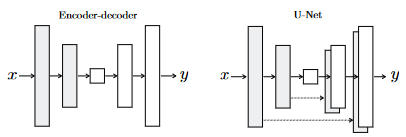
\includegraphics[width=0.7\linewidth]{./images/unet.png}
	\caption{Schematische Darstellung der U-Net-Architektur. Die Architektur besteht aus einem Encoder-Teil (links), einem Decoder-Teil (rechts) und Skip-Verbindungen zwischen korrespondierenden Schichten.}
	\label{fig:unet}
\end{figure}

\subsection{Anwendungen von Pix2Pix}
Pix2Pix ist eine fortschrittliche Methode für Bild-zu-Bild-Übersetzungsaufgaben und hat eine breite Palette von Anwendungen in der Bildverarbeitung.\newline
Ein markantes Anwendungsbeispiel ist die Umwandlung von architektonische Entwürfe oder Zeichnungen in realistische Gebäudefotos. Besonders eindrucksvoll ist diese Anwendung beim CMP Facades-Datensatz, wo aus simplen Fassadenzeichnungen detailreiche Gebäudebilder generiert werden. \cite{PhillipIsola.}
\newline
Im Bereich der Fotografie wird Pix2Pix verwendet, um Schwarz-Weiß-Fotos in farbige Bilder zu konvertieren, was besonders bei der Restaurierung alter Fotografien von Bedeutung sein kann \cite{PhillipIsola.}.
\newline
Die Transformation von Tagesaufnahmen in Nachtbilder ist eine weitere beeindruckende Leistung von Pix2Pix sowie die Umwandlung von Thermalaufnahmen in Farbfotos \cite{PhillipIsola.}.
\newline
Schließlich wird Pix2Pix auch zur Vervollständigung von Fotos mit fehlenden Pixeln verwendet, beispielsweise um unvollständige Bilder, die aus Paris StreetView stammen, zu reparieren und zu vervollständigen \cite{PhillipIsola.}.
\newline
Jedoch kann Pix2Pix auch bei medizinischen Anwendungen, insbesondere in der Augenheilkunde, hilfreich sein. Hier wird Pix2Pix für die Post-Interventions-\\Prognose eingesetzt, um zu zeigen, wie sich die Netzhaut nach einer Anti-VEGF-\\Injektionsbehandlung verändert. Dies basiert auf Bildern, die vor der Injektion bei Patienten mit exsudativer altersbedingter Makuladegeneration aufgenommen wurden. Durch diese Technik können Ärzte und Patienten eine Vorstellung davon bekommen, welche Veränderungen im Auge nach der Behandlung zu erwarten sind \cite{AramYouJinKukKimIkHeeRyuTaeKeunYoo.2022}.

\section{CycleGAN}
CycleGAN, das 2017 von Jun-Yan Zhu et al. vorgestellt wurde, stellt eine neue Entwicklung im Bereich des maschinellen Lernens und insbesondere der Bildübersetzung zwischen unpaaren Domänen dar. Es erweitert die Pix2Pix-Architektur durch die Einführung einer Zykluskonsistenz-Verlustfunktion (Cycle Consistency Loss), die sicherstellt, dass das Originalbild nach einem Übersetzungs- und Rückübersetzungszyklus erhalten bleibt. Der Generator $G$ transformiert Bilder aus der Domäne $X$ in die Domäne $Y$, während der Generator $F$ den umgekehrten Prozess durchführt. Diese Transformationen werden ohne gepaarte Trainingsdaten durchgeführt.

\subsection{CycleGAN - Kernkonzepte}
\chapter*{Cycle GAN}

CycleGAN ist ein leistungsstarkes Modell im Bereich des maschinellen Lernens, das darauf abzielt, Bildübersetzungen zwischen verschiedenen Domänen ohne die Notwendigkeit für gepaarte Daten durchzuführen. Diese Technik wurde erstmals 2017 von Jun-Yan Zhu et al. in ihrer bahnbrechenden Arbeit "Unpaired Image-to-Image Translation using Cycle-Consistent Adversarial Networks" vorgestellt. Dieses Kapitel widmet sich der Funktionsweise von CycleGAN und seinen vielfältigen Anwendungen.

\subsection*{Funktionsweise von CycleGAN}

CycleGAN basiert auf dem GAN-Prinzip. Der Generator erzeut Bilder, während der Diskriminator zwischen den echten und generierten Bilder unterscheiden muss. Im Falle von CycleGAn wird das Modell erweitert, um die Übersetzung zwischen zwei Domänen $X$ und $Y$ zu ermöglichen. 

\subsection*{Generator}

\subsection*{Diskriminator}

\subsection*{Cycle - Konsistenz}

\subsection*{Verlustfunktionen}


\section{Convolutional Layers}
Convolutional Layers repräsentieren eine fundamentale Komponente innerhalb neuronaler Netzwerke, insbesondere im Kontext der Verarbeitung von Bildinformationen. Diese Schicht nutzt Convolution-Operationen, um durch Faltung von Eingabedaten mit Filterkernen lokale Muster zu identifizieren. Die Filterkerne, üblicherweise in Größen wie 3x3, 7x7 oder 9x9, fungieren als kleine Arrays und dienen der Extraktion spezifischer Merkmale im Bild.

Die Funktionsweise dieser Schicht basiert auf der schrittweisen Verschiebung der Filterkerne über das Eingangsbild. An den jeweiligen Pixelpositionen erfolgt eine präzise elementweise Multiplikation, gefolgt von einer anschließenden Summation aller resultierenden Werte. Diese berechneten Werte werden dann in den korrespondierenden Positionen der Feature Map eingetragen, wie in der Abbildung \ref{fig:convolutionalLayer} veranschaulicht. Durch diesen Prozess gewinnen tiefere Schichten des Netzwerks die Fähigkeit, zunehmend komplexe und abstrakte Informationen auf höheren Ebenen der Hierarchie zu repräsentieren.

\begin{figure}[ht]
	\centering
	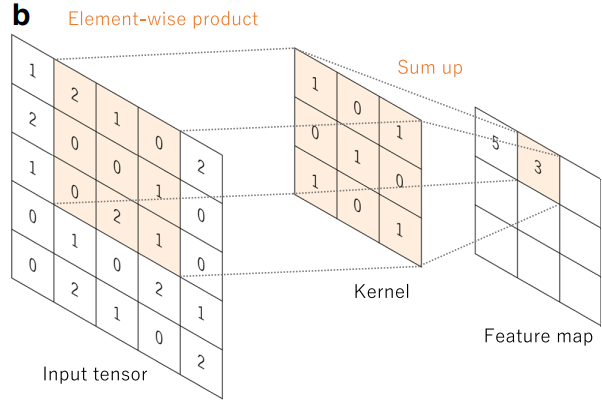
\includegraphics[width=0.5\linewidth]{./images/convolutionalLayer.png}
	\caption{Beispiel einer Convolutional-Operation mit einem 3x3 Kernel und Stride 1 \cite{Yamashita.2018}}
	\label{fig:convolutionalLayer}
\end{figure}

Die Verwendung verschiedener Kernels, sowohl in Bezug auf Größe als auch Anzahl, erlaubt die Extraktion vielfältiger Merkmale wie Kanten oder Texturen. Diese Flexibilität befähigt das Netzwerk, auf unterschiedlichste visuelle Strukturen ansprechend zu reagieren \cite{Yamashita.2018}.

Zusätzlich fungieren die Kernels als Subsampling-Mechanismus, bedingt durch die begrenzte Ausdehnung der Convolution-Operation bis zum Bildrand. Die Wahl der Strides, als die Distanz zwischen zwei verschobenen Kernelpositionen, beeinflusst diesen Subsampling-Effekt. Die Anwendung von Padding, um das Bild vor jeder Convolution zu vergrößern, kann dazu beitragen, ungewollte Unterabtastung (Downsampling) zu minimieren.

Ein wesentlicher Vorzug von Convolutional Layers besteht in der signifikanten Reduzierung der zu trainierenden Parameter und der Komplexität des Modells. Dies führt zu einer verbesserten Effizienz, da weniger Gewichte optimiert werden müssen, und trägt zur Prävention von Overfitting bei \cite{Yamashita.2018,OShea.2015}.

Die Ergebnisse der Convolutional Layer werden anschließend durch eine nicht-lineare Aktivierungsfunktion weitergereicht, um die Fähigkeit des Netzwerks zur Modellierung komplexer, nicht-linearer Zusammenhänge zu verbessern. Die Einbeziehung einer Aktivierungsfunktion, wie beispielsweise der ReLU (Rectified Linear Unit), ermöglicht es dem Netzwerk, nicht-linear separierbare Muster und Merkmale zu erfassen. Ohne Aktivierungsfunktionen würden die Convolutional Layers nur lineare Transformationen durchführen, was die Lernfähigkeit des Modells deutlich einschränken würde \cite{Sharma.2017}.

\section{Bibliotheken}
\subsection{Tensorflow}
TensorFlow ist ein weit verbreitetes Open-Source-Framework, das für maschinelles Lernen und tiefe neuronale Netzwerke eingesetzt wird\footnote{https://www.tensorflow.org/}. Es bietet eine umfangreiche Plattform zur Entwicklung und Umsetzung von Modellen in verschiedenen Anwendungsbereichen, darunter Bilderkennung und natürliche Sprachverarbeitung. Die Architektur von TensorFlow ermöglicht das Erstellen komplexer maschineller Lernanwendungen und stellt umfassende Tools und Bibliotheken zur Verfügung, um den gesamten Entwicklungsprozess zu unterstützen. Darüber hinaus profitiert TensorFlow von einer aktiven und engagierten Community, die kontinuierlich zur Weiterentwicklung des Frameworks beiträgt\footnote{https://github.com/tensorflow/tensorflow}.

\subsection{Keras}
Ursprünglich als eigenständiges Framework konzipiert und seit TensorFlow 2.0 in die TensorFlow Core API integriert, fungiert Keras als Open-Source-API zur Modellierung von Strukturen im Bereich des Deep Learning\footnote{https://www.tensorflow.org/guide/keras}. Diese Bibliothek, die in der Programmiersprache Python implementiert ist, umfasst sämtliche Phasen des maschinellen Lern-Workflows. Beginnend mit der Datenverarbeitung ermöglicht sie eine Fortführung bis zur präzisen Abstimmung der Hyperparameter während des Trainingsprozesses. Die Keras-Prinzipien zeichnen sich durch Einfachheit, Flexibilität und Leistungsfähigkeit aus und ermöglichen es den Anwendern, die Skalierbarkeit und plattformübergreifenden Fähigkeiten der TensorFlow-Plattform zu nutzen\footnote{https://keras.io/about/}.

\subsection{Matplotlib}
Matplotlib ist eine weit verbreitete und leistungsstarke Python-Bibliothek zur Erstellung von statischen, interaktiven und animierten Visualisierungen. Entwickelt von John D. Hunter im Jahr 2003, hat sich Matplotlib zu einem Standardwerkzeug in der Datenvisualisierung und wissenschaftlichen Forschung entwickelt\footnote{https://matplotlib.org/}.
\chapter{Hauptteil - 1}
Hier wird der Inhalt der Arbeit präsentiert.
\chapter{Hauptteil - 2}
Hier wird der Inhalt der Arbeit präsentiert.
\chapter{Hauptteil - 3}
Hier wird der Inhalt der Arbeit präsentiert.
\chapter{Evaluation}
\section{Bewertungskriterien}
\subsection{Diskriminator-Verlust}
Der Diskriminator-Verlust ist ein wesentliches Maß für die Effektivität des Diskriminators in einem GAN-Modell. Ein niedriger Diskriminator-Verlust bedeutet, dass der Diskriminator erfolgreich zwischen echten und generierten Bildern unterscheiden kann. Im Kontext eines GANs zeigt ein abnehmender Diskriminator-Verlust über die Epochen hinweg, dass der Diskriminator zunehmend besser darin wird, die Authentizität der Bilder zu beurteilen. Ein hoher Diskriminator-Verlust weist hingegen darauf hin, dass das Modell Schwierigkeiten hat, echte von generierten Bildern zu unterscheiden, was ein Indikator für Verbesserungspotenzial im Training oder der Modellarchitektur sein könnte.

\subsection{Generator-Verlust}
Der Generator-Verlust ist ein Indikator für die Fähigkeit des Generators, Bilder zu erzeugen, die vom Diskriminator als echt eingestuft werden. Ein hoher Generator-Verlust deutet darauf hin, dass der Generator die realen Daten noch nicht effektiv nachahmen kann, während ein niedriger Generator-Verlust ein Zeichen dafür ist, dass die generierten Bilder den echten immer ähnlicher werden. Im Verlauf des Trainings sollte der Generator-Verlust tendenziell abnehmen, was darauf hindeutet, dass der Generator lernt, überzeugendere Bilder zu produzieren.

\subsection{Diskriminator Genauigkeit}
Die Diskriminator-Genauigkeit gibt an, wie oft der Diskriminator korrekt zwischen echten und gefälschten Bildern unterscheidet. Eine hohe Genauigkeit bedeutet, dass der Diskriminator effektiv arbeitet, während eine niedrige Genauigkeit auf Probleme bei der Unterscheidung hinweisen kann. Es ist wichtig, ein Gleichgewicht zu finden, denn eine zu hohe Genauigkeit kann darauf hindeuten, dass der Diskriminator die generierten Bilder zu leicht erkennt, was auf ein Problem mit dem Generator hinweisen könnte.\newline
In einem ideal funktionierenden GAN sollte der Diskriminator eine Genauigkeit von etwa 50$\%$ erreichen. Das bedeutet, dass der Diskriminator die echten von dem generierten Bildern nur zufällig unterscheiden bzw. nicht mehr zuverlässig unterscheiden kann, was zeigt dass das GAN gut trainiert wurde.

\subsection{SSIM-Score (Structural Similarity Index)}
Der SSIM-Score ist ein Maß für die visuelle Ähnlichkeit zwischen den generierten Bildern und den entsprechenden Originalbildern. Er bewertet die Bildqualität anhand von Faktoren wie Helligkeit, Kontrast und Struktur. Ein hoher SSIM-Wert deutet darauf in, dass die generierten Bilder den echten Bildern sehr ähnlich sind, was ein Zeichen für eine hohe Bildqualität ist. Ein niedriger SSIM-Wert kann auf deutliche Unterschiede in der visuellen Struktur hinweisen, was Verbesserungsbedarf im Generator-Training oder in der Modellarchitektur signalisiert.

\section{Pix2Pix: Ergebnisse und objektive Bewertung}
 Diese Flexibilität in der Kanalverarbeitung ermöglicht eine breitere Anwendung des Pix2Pix-Modells auf verschiedene Bildtypen. Die Bilder müssen nicht in einer bestimmten Weise vorverarbeitet werden, da das Modell direkt auf den Rohpixeln arbeitet. Diese Flexibilität in der Kanalverarbeitung und die Fähigkeit, direkt auf Rohpixeln zu arbeiten, unterstreichen die Vielseitigkeit des Pix2Pix-Modells.
  Durch empirische Tests hat sich herausgestellt das eine initiale Lernrate von 0.0002 und die Momentum-Parameter von $\beta1$ = 0.5 und $\beta$ = 0.999 optimal sind, um die Balance zwischen Lerngeschwindigkeit und Stabilität des Trainingsprozesses zu optimieren. Auch die Wahl einer kleinen Batchgröße, typischerweise 1, spielt eine entscheidende Rolle, um die Trainingseffizienz zu maximieren und qualitativ hochwertige Ergebnisse zu erzielen. Diese spezifischen Einstellungen der Trainingsparameter tragen maßgeblich dazu bei, das Potenzial des Pix2Pix-Modells voll auszuschöpfen.\cite{PhillipIsola.}.\newline
  Für den Generator und den Diskriminator, wird der Adam-Optimierer mit einer Lernrate von 0.0002 und den Momentum-Parametern $\beta$1 = 0.5 und $\beta$2 = 0.999 verwendet. Diese Einstellungen einen guten Kompromiss zwischen der Lerngeschwindigkeit und der Stabilität des Trainingsprozesses zu finden. Die Batchgröße ist im Code auf 1 gesetzt. Eine kleine Batchgröße kann zu einer höheren Stabilität im Trainingsprozess beitragen. Der Hyperparameter $LAMBDA$ wird verwendet, um das Gewicht des L1-Verlustes im Generatorverlust zu steuern. Ein hoher Wert von $LAMBDA$ betont die Bedeutung der Inhaltsähnlichkeit zwischen den generierten und den Zielbildern. Die Anzahl der Trainingsepochen ist auf 450 gesetzt, was darauf hindeutet, dass das Modell eine umfangreiche Trainingsdauer durchläuft, um eine optimale Leistung zu erreichen.
\section{CycleGAN: Ergebnisse und objekte Bewertung}
\section{Vergleich und Bewertung von Pix2Pix und CycleGAN}
\section{Vergleich von Pix2Pix und CycleGAN}
- Matching Paare von Bildern sind ebenfalls für das Training nicht nötig (crewall)
- Macht die Datenvorbereitung einfacher und öffnet neue Techniken für Applikationen (crewall)
\chapter{Fazit und Ausblick}
Hier wird ein Fazit und ein Ausblick gegeben.

\section{Fazit}
Im Zuge dieses Teamprojekts wurden zentrale Forschungsfragen im Bereich der Bildverarbeitung mit Generative Adversarial Networks (GANs) untersucht und beantwortet. Dabei standen insbesondere die Frameworks Pix2Pix und CycleGAN im Fokus, um die vielfältigen Anwendungsmöglichkeiten und Herausforderungen von GANs zu beleuchten. Durch die praktische Implementierung und das Training der Modelle Pix2Pix und CycleGAN auf einem spezifischen Datensatz konnten wir die Leistungsfähigkeit und Grenzen dieser Technologien demonstrieren. Die Ergebnisse zeigen, dass beide Modelle effektiv in der Bild-zu-Bild-Übersetzung sind, sich jedoch in ihren Stärken und Herausforderungen unterscheiden.

Während Pix2Pix für seine Effizienz bei gepaarten Trainingsdaten bekannt ist, demonstriert CycleGAN seine Stärke in der Zykluskonsistenz bei ungepaarten Daten. Die Analyse der SSIM-Scores und Diskriminatorgenauigkeiten und weiterer Metriken beider Modelle hat einen tiefgreifenden Einblick in ihre Fähigkeit zur Erzeugung qualitativ hochwertiger Bilder ermöglicht. Besonders auffällig war die kontinuierliche Verbesserung der Bildqualität bei CycleGAN im Laufe des Trainings sowie die Notwendigkeit der sorgfältigen Anpassung der Trainingsparameter bei Pix2Pix und CycleGAN. Diese Erkenntnisse unterstreichen die Bedeutung einer gezielten und durchdachten Konfiguration der Trainingsparameter für die erfolgreiche Anwendung von GANs in der Bildverarbeitung.

\section{Ausblick}
Der Ausblick für die weitere Forschung und Anwendung von Generative Adversarial Networks (GANs) im Bereich der Bildverarbeitung ist vielversprechend und bietet zahlreiche Möglichkeiten für Innovationen. Die Ergebnisse dieses Projekts legen nahe, dass zukünftige Arbeiten sich darauf konzentrieren könnten, die Effizienz und Genauigkeit von GAN-Modellen weiter zu verbessern, insbesondere in Bereichen, in denen hochpräzise Bild-zu-Bild-Übersetzungen erforderlich sind.

Des Weiteren könnte die Erforschung neuer Anwendungsbereiche, in denen GANs bisher noch nicht eingesetzt wurden, neue Horizonte eröffnen. Dies könnte die Entwicklung maßgeschneiderter Lösungen für spezifische Branchen oder kreative Prozesse beinhalten. Auch die Auswirkungen unterschiedlicher Datensätze und die Entwicklung von GANs, die effektiv mit weniger oder ungepaarten Daten arbeiten können, sind vielversprechende Forschungsfelder. Letztlich könnte die Erweiterung der ethischen und rechtlichen Rahmenbedingungen, insbesondere in Bezug auf die Verwendung generierter Bilder, eine Schlüsselrolle spielen, um das volle Potenzial von GANs in einer verantwortungsbewussten und nachhaltigen Weise zu nutzen.

\chapter*{Generative Adversial Network}


Generative Adversial Networks, kurz GANs, sind eine aufstrebende Technologie im Bereich des maschinellen Lernens und der künstlichen Intelligenz. Inspiriert von Ian Goodfellow und seinen Kollegen im Jahr 2014, bieten GANs eine effiziente Möglichkeit, tiefe Repräsentationen von Daten zu erlernen, ohne dass große Mengen an annotierten Trainingsdaten benötigt werden. 
Dies wird durch die Verwendung von Backpropagation und den Wettbewerb zwischen zwei neuronalen Netzen - dem Generator und dem Diskriminator - erreicht. 
Daraus ergeben sich zahlreiche neue Ansätze zur Generierung realistischer Inhalte. 
Die Anwendungen reichen von der Bildgenerierung bis hin zur Superauflösung und Textgenerierung.

\section*{Verfahren}
Der Generator und der Diskriminator sind die Hauptkomponenten eines GAN. Die beiden neuronalen Netze werden gleichzeitig trainiert und konkurrieren miteinander, wobei der Generator versucht, den Diskriminator zu täuschen, indem er synthetische Inhalte erzeugt. Um die Glaubwürdigkeit des Generators zu erhöhen, so dass der Diskriminator nicht mehr zwischen den Eingaben unterscheiden kann, wird das gesamte Netz trainiert. Die Netze werden in der Regel als Mehrschichtnetze implementiert, die aus Faltungsschichten und vollständig verbundenen Schichten bestehen.

\subsection*{Generator}
Der Generator dient zur Erzeugung künstlicher Daten wie Bilder und Texte. 
Der Generator ist nicht mit dem realen Datensatz verbunden und lernt daher nur durch die Interaktion mit dem Diskriminator. Wenn der Diskriminator nur noch 50\% der Eingaben richtig vorhersagt, gilt der Generator als optimal.

\subsection*{Diskriminator}
Die Unterscheidung zwischen echten und unechten Eingaben ist Aufgabe des Diskriminators. Der Diskriminator kann sowohl künstliche als auch reale Daten verwenden. 
Wenn der Diskriminator nicht mehr richtig unterscheiden kann, wird er als konvergierend bezeichnet. Andernfalls wird er als optimal bezeichnet, wenn seine Klassifizierungsgenauigkeit maximiert ist. Im Falle eines optimalen Diskriminators wird das Training des Diskriminators gestoppt und der Generator trainiert alleine weiter, um die Genauigkeit des Diskriminators wieder zu verbessern.

\subsection*{Training}
Durch das Finden von Parametern für beide Netze wird das Training durchgeführt. Ziel ist die Optimierung beider Netze durch Anwendung von Backpropagation zur Verbesserung der Parameter. Das Training wird oft als schwierig und instabil beschrieben, da es einerseits schwierig erscheint, beide Modelle konvergieren zu lassen. Auf der anderen Seite kann der Generator sehr ähnliche Muster für verschiedene Eingaben erzeugen, und der Diskriminatorverlust kann schnell gegen Null konvergieren, so dass es keinen zuverlässigen Weg für die Gradientenaktualisierung zum Generator gibt. 
Zur Lösung dieser Probleme wurden verschiedene Ansätze vorgeschlagen, wie z.B. die Verwendung heuristischer Verlustfunktionen. Eine weitere Möglichkeit, die von Sonderby et al. vorgeschlagen wurde, besteht darin, den Datensatz vor der Verwendung zu verrauschen.

\section*{Anwendung}
GAN wurde ursprünglich für unüberwachtes maschinelles Lernen entwickelt. Die Architektur liefert jedoch ebenso gute Ergebnisse beim halbüberwachten Lernen und beim Reinforcement Learning. 
Aus diesem Grund wird sie in einer Vielzahl von Bereichen wie dem Gesundheitswesen, dem Maschinenbau und dem Bankwesen eingesetzt. Beispielsweise wird GAN in der Medizin zur Erkennung und Behandlung chronischer Krankheiten eingesetzt. Aber auch die Identifikation von 3D-Objekten und die Generierung von realen Bildern und Texten ist durch den Einsatz von GANs möglich.

\section*{Limitationen}
Die Tatsache, dass ein Generative Adversial Network in der Lage ist, Inhalte zu erzeugen, die nahezu identisch mit realen Inhalten sind, kann in der realen Welt zu Problemen führen, insbesondere bei der menschlichen Bildsynthese. Diese Bilder können von Betrügern verwendet werden, um falsche Profile in sozialen Medien zu erstellen. 
Auch dies kann durch den Einsatz von GANs verhindert werden, indem einzigartige und pragmatische Bilder von nicht existierenden Personen erzeugt werden.


%%%======================================================================================

% Anhang
\appendix
\kapitelbalken{akb}
\chapter{Anhang - Code}

Dieser Abschnitt enthält die wichtigsten Funktionen, die in der Implementierung verwendet werden. 
Hier finden sich auch die fehlenden Funktionen aus dem Kapitel 'Lösungsbeschreibung'.

\section*{Datenvorverarbeitung}
\begin{lstlisting}[language=pyhaff, caption={Lesen eines Bildes (CycleGAN Implementierung)}, label={cod:imageLoading}]
def load_image(image_path):
    image = tf.io.read_file(image_path)
    image = tf.io.decode_jpeg(image, channels=3)
    image = tf.cast(image, tf.float32)
    return image
\end{lstlisting}

\newpage
%% MARCEL
\section*{Pix2Pix}
\lstinputlisting[language=pyhaff, caption=Pix2Pix Trainingsfunktion, label={cod:pix2pixTrain}]{code/Pix2Pix_Trainingfunktion.txt}

\newpage
\section*{CycleGAN}
\begin{lstlisting}[language=pyhaff, caption={Residualblock Implementierung}, label={cod:residual}]
def residual_block(x, filters):
    shortcut = x
    x = tf.keras.layers.Conv2D(filters, kernel_size=3, strides=1, padding='same')(x)
    x = InstanceNormalization(axis=-1)(x)
    x = tf.keras.layers.LeakyReLU()(x)
    x = tf.keras.layers.Conv2D(filters, kernel_size=3, strides=1, padding='same')(x)
    x = InstanceNormalization(axis=-1)(x)
    x = tf.keras.layers.Concatenate()([x, shortcut])
    return x
\end{lstlisting}

\begin{lstlisting}[language=pyhaff, caption={Convolutional Block in CycleGAN}, label={cod:cycleGANConvolutional}]
def convolutional_layer(x, filters, kernel_size=3, strides=2):
    x = tf.keras.layers.Conv2D(filters, kernel_size=kernel_size, strides=strides, padding='same')(x)
    InstanceNormalization(axis=-1)(x)
    x = tf.keras.layers.LeakyReLU()(x)
    return x
\end{lstlisting}

\newpage
\begin{lstlisting}[language=pyhaff, caption={Transpose Convolutional Block in CycleGAN}, label={cod:cycleGANTransposeConv}]
def t_convolutional_layer(x, filters, kernel_size=3, strides=2):
    x = tf.keras.layers.Conv2DTranspose(filters, kernel_size=kernel_size, strides=strides, padding='same')(x)
    InstanceNormalization(axis=-1)(x)
    x = tf.keras.layers.LeakyReLU()(x)
    return x
\end{lstlisting}

\begin{lstlisting}[language=pyhaff, caption={Adversarieller Verlust des Generators in CycleGAN}, label={cod:cycleGANadversarialLoss}]
def generator_adversarial_loss(generated):
    return loss_obj(tf.ones_like(generated), generated)
\end{lstlisting}

\begin{lstlisting}[language=pyhaff, caption={Zykluskonsistenz Verlust in CycleGAN}, label={cod:cycleLoss}]
def cycle_loss(real_image, cycled_image):
  loss1 = tf.reduce_mean(tf.abs(real_image - cycled_image))
  return LAMBDA * loss1
\end{lstlisting}

\begin{lstlisting}[language=pyhaff, caption={Identitätsverlust in CycleGAN}, label={cod:identityLoss}]
def identity_loss(real_image, same_image):
  loss = tf.reduce_mean(tf.abs(real_image - same_image))
  return LAMBDA * 0.5 * loss
\end{lstlisting}

\newpage
\lstinputlisting[language=pyhaff, caption={CycleGAN Trainingsfunktion, Teil 1}, label={cod:cycleTrain1}]{code/CycleGan_Training1.txt}
\newpage
\lstinputlisting[language=pyhaff, caption={CycleGAN Trainingsfunktion, Teil 2}, label={cod:cycleTrain2}]{code/CycleGan_Training2.txt}

\newpage
\section*{Training und Hyperparameter}
\begin{lstlisting}[language=pyhaff, caption={Speicherung der Metriken in CSV-Datei}, label={cod:csvSave}]
def save_losses(epoch, gen_loss, disc_loss, disc_accuracy, ssim):
  with open(losses_path, 'a') as f:
    writer = csv.writer(f)
    writer.writerow([epoch, gen_loss.result().numpy(), disc_loss.result().numpy(), disc_accuracy, ssim])
\end{lstlisting}

\begin{lstlisting}[language=pyhaff, caption={Berechnung des SSIM-Score}, label={cod:ssim}]
def calculate_ssim(generator, dataset, num_samples=10):
    ssim_values = []
    for input_image, target_image in dataset.take(num_samples):
        prediction = generator(input_image, training=False)
        ssim_value = tf.image.ssim(prediction, target_image, max_val=2.0)
        ssim_values.append(ssim_value)
    return tf.reduce_mean(ssim_values)
\end{lstlisting}

\newpage

\begin{lstlisting}[language=pyhaff, caption={Ausschnitt zur Erstellung einer Verlaufskurve (CycleGAN Implementierung)}, label={cod:curve}]
def plot_curve(name, epoch, col2, col_name, num_curves=1):
    path = f"./satelite/try1/Curves/{name}.jpg"
    if not os.path.exists("./satelite/try1/Curves/"):
        os.makedirs("./satelite/try1/Curves/")
    for i in range(num_curves):
        plt.plot(epoch, col2.iloc[:, i], label=col_name[i])
    plt.xlabel('Epoche')
    plt.ylabel(name)
    plt.title(f'Epoche vs {name}')
    plt.legend()
    plt.savefig(path)
    plt.show()

def save_curves():
    df = pd.read_csv('./satelite/try1/losses.csv')
    epoche = df.iloc[:, 0]
    gen_loss = df.iloc[:, [1, 2]]
    plot_curve("Generator_Verlust", epoche, gen_loss, ["Generator_F_Verlust", "Generator_G_Verlust"], 2)
\end{lstlisting}
\chapter{Anhang - Dokumentationen}
Hier sehen Sie die gesamten Dokumentationen zu den erstellten Programmen.




% muss stehen bleiben, da sonst die Kapitelbalken nicht bei allen Seiten von Anhang B auftauchen
\cleardoublepage

% deaktiviert die chapterthumbs wieder, sodass sie nicht in den Verzeichnissen auftauchen.
\lohead[]{}

% Verzeichnisse
\Ifpdfoutput{\ihead[]{}}{}
% Hier werden alle Verzeichnisse erzeugt, die am Ende der Arbeit aufgelistet werden.
% mit diesem Befehl wird dem Inhaltsverzeichniss das Kapitel "Verzeichnisse hinzugefügt
\addcontentsline{toc}{chapter}{Verzeichnisse}

\addcontentsline{toc}{section}{Literaturverzeichnis}
\nocite{*}						% damit die ganze Literatur im Verzeichniss erscheint, auch, wenn diese nicht zitiert wurde! 
\bibliographystyle{alphadin}	% Stil des Literaturverzeichnisses
\bibliography{literatur}		% Literaturverzeichnis
\cleardoublepage

% Erstellt das Abbildungsverzeichnis
\listoffigures
\addcontentsline{toc}{section}{Abbildungsverzeichnis}   % Abbildungsverzeichnis	
\cleardoublepage

% Erstellt das Tabellenverzeichnis - Bei Bedarf einfügen
\listoftables
\addcontentsline{toc}{section}{Tabellenverzeichnis}		% Tabellenverzeichnis
\cleardoublepage

% Erstellt das Code-Auszugs-Verzeichnis - Bei Bedarf einfügen
\lstlistoflistings
\addcontentsline{toc}{section}{Code-Auszugs-Verzeichnis}% Code-Auszugs-Verzeichnis
\cleardoublepage

% Glossar
\addcontentsline{toc}{section}{Glossar}
\chapter*{Glossar}

\begin{itemize}
    \item \textbf{C++}:\\ Hardwarenahe, objektorientierte Programmiersprache.
	\item \textbf{HTML}:\\ Hypertext Markup Language - textbasierte Auszeichnungssprache zur Strukturierung elektronischer Dokumente.
	\item \textbf{HTTP}:\\ Hypertext Transfer Protocol - Protokoll zur Übertragung von Daten auf der Anwendungssicht über ein Rechnernetz.
	\item \textbf{iARS}:\\ innovative Audio Response System - System mit zwei Applikationen (iARS-master-App; iARS-student-App), dass sich zum Einsetzten von e-TR-ainer-Inhalten in Vorlesungen eignet.
	\item \textbf{ISO}:\\ Internationale Vereinigung von Normungsorganisationen.
	\item \textbf{JavaScript}:\\ Skriptsprache zu Auswertung von Benutzerinteraktionen.
	\item \textbf{Konstruktor}:\\ Beim Erzeugen einer Objektinstanz aufgerufene Methode zum Initialisieren von Eigenschaften.
	\item \textbf{MySQL}:\\ Relationales Datenbankverwaltungssystem.
	\item \textbf{OLAT}:\\ Online Learning and Training - Lernplattform für verschiedene Formen von webbasiertem Lernen.
	\item \textbf{OOP}:\\  Objektorientierte Programmierung - Programmierparadigma, nach dem sich die Architektur eine Software an realen Objekten orientiert.
	\item \textbf{Open Source}:\\ Software, die öffentlich von Dritten eingesehen, geändert und genutzt werden kann.
	\item \textbf{PHP}:\\ Skriptsprache zur Erstellung von Webanwendungen.
	\item \textbf{Python}:\\ Skript- und Programmiersprache, die unter Anderem objektorientiertes Programmieren ermöglicht.
	\item \textbf{Shell}:\\ Shell oder auch Unix-Shell - traditionelle Benutzerschnittstelle von Unix-Betriebssystemen
	\item \textbf{Spyder}:\\ Entwicklungsumgebung für wissenschaftliche Programmierung in der Programmiersprache Python.
	\item \textbf{SymPy}:\\ Python-Bibliothek für symbolische Mathematik.
\end{itemize} 

\end{document}